\documentclass{article}

\usepackage{Sweave}
\begin{document}
\Sconcordance{concordance:analyzePower.tex:analyzePower.Rnw:%
1 2 1 1 0 7 1 1 14 5 0 1 2 1 3 5 0 1 2 1 3 5 0 1 2 3 1}


\title{Analyse der Akkulaufzeit}
\maketitle

\begin{itemize}
\item Beschleunigungsdaten 1x pro Sekunde speichern, nur Beschleunigungsdaten aufgezeichnet
\begin{Schunk}
\begin{Soutput}
[1] "36826"
\end{Soutput}
\end{Schunk}
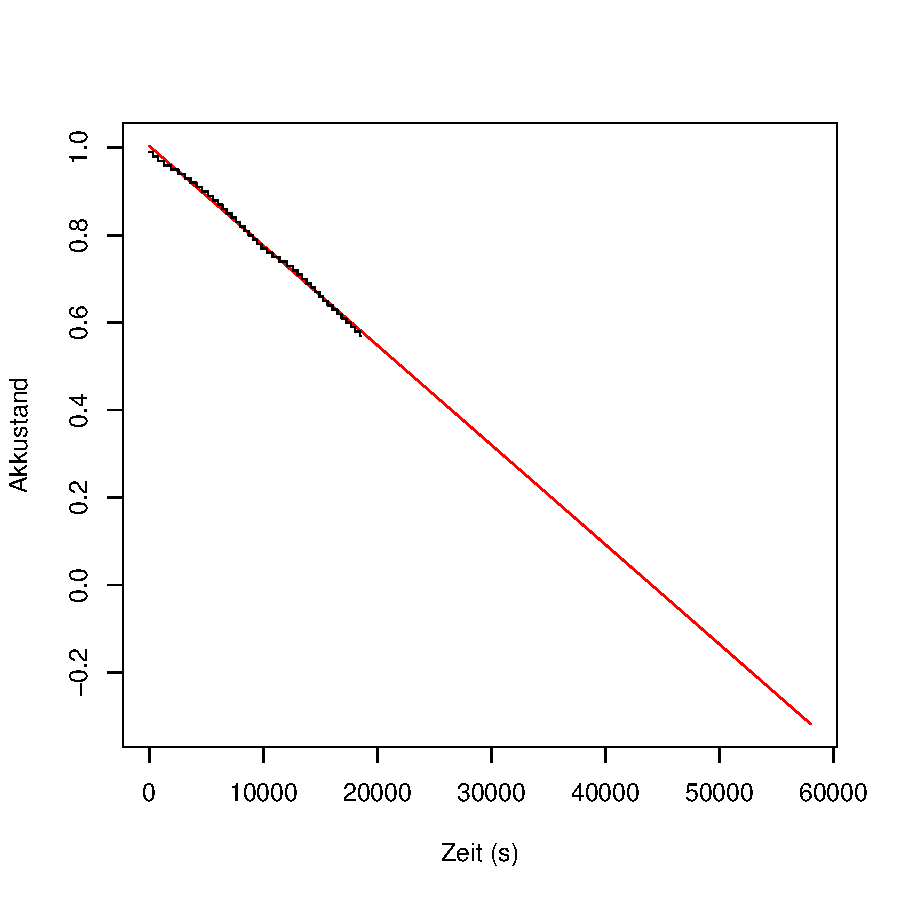
\includegraphics{analyzePower-001}
\item Beschleunigungsdaten 1x pro Minute speichern, nur Beschleunigungsdaten aufgezeichnet
\begin{Schunk}
\begin{Soutput}
[1] "39337"
\end{Soutput}
\end{Schunk}
\includegraphics{analyzePower-002}
\item Lagedaten 1x pro Sekunde aufzeichnen, nur Lagedaten aufgezeichnet
\begin{Schunk}
\begin{Soutput}
[1] "38808"
\end{Soutput}
\end{Schunk}
\includegraphics{analyzePower-003}
\item Lagedaten und Beschleunigungsdaten 1x pro Sekunde aufgezeichnet
\begin{Schunk}
\begin{Soutput}
[1] "36163"
\end{Soutput}
\end{Schunk}
\includegraphics{analyzePower-004}

\end{itemize}

\end{document}
